\raggedright
A botnet is a network of inter-connected and infected devices. These devices, referred to as bots or 'zombies', become
infected by malware distributed to purposely take control of them. Botnets are then primarly used to distribute the
same or other malware, or launch Distributed Denial-of-Service (DDoS) attacks. The individual or group that develops
and/or runs the botnet is referred to as the botmaster. They constantly add bots to the network by distributing
bot malware to infect new devices.

\subsection{Botnet Architectures}

Botnet mainly use a client-server architecture, but some instead use a peer-to-peer (P2P) architecture\textsuperscript{\cite{fedynyshyn2011detection}}. In a client-server
architecture, there is a centralized computer that issues commands to, and receives information from, the infected bots.
It frequently consists of several servers and other technical components. Bots report back to the botnet's command and control
(C\&C) server, whilst the C\&C issues instructions to the bots to perform illegitimate tasks.

Unlike the client-server architecture, a P2P architecture is a \textit{decentralized} network of bots - with no command and control server.
The bots act as both a command distribution server, as well as a client that receives commands. The random structure of the botnet
further obfuscates itself and increases protection against it being taken down. Although they cannot be easily identified,
the botmaster cannot easily monitor command delivery.

\vspace{0.5cm}

\begin{figure}[h]
	\begin{subfigure}{0.5\textwidth}
		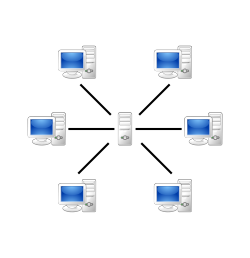
\includegraphics[width=0.9\linewidth, height=5cm]{img/botnet_client_server.png} 
		\caption{Client-Server Botnet}
	\end{subfigure}
	\begin{subfigure}{0.5\textwidth}
		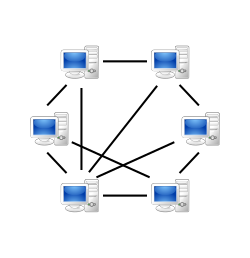
\includegraphics[width=0.9\linewidth, height=5cm]{img/botnet_p2p.png}
		\caption{Peer-to-Peer Botnet}
	\end{subfigure}
	\caption{Client-Server and Peer-to-Peer Botnets\textsuperscript{\cite{botnetwikipedia}}}
\end{figure}

\subsection{Classification}

Command and control botnets can be classed under three main types\textsuperscript{\cite{fedynyshyn2011detection}}:
\begin{enumerate}
	\item Internet Relay Chat (IRC) botnets
	\item HTTP botnets
	\item P2P botnets
\end{enumerate}

IRC-based botnets\textsuperscript{\cite{dubendorfer2004analysis}} use a \textit{push-based} model in which the botmaster pushes
new commands to the botnet, through the use of an IRC channel, where bots
respond directly to the commands given.

HTTP-based botnets use a \textit{pull-based} model of communication, where the
bots individually poll the command and control server to request new commands
to execute.

P2P botnets are \textit{decentralized}, where the bots themselves operate as a command
distribution server, as well as the client that receives commands.

\vspace{0.5cm}

Many botnets use a DNS technique called \textbf{fast flux}\textsuperscript{\cite{nazario2008net}}. This allows the
botnet to hide their central command and control server. This does not apply
to P2P botnets due to the nature of the botnet architecture. This adds an extra
layer of protection against takedowns.